\documentclass[tikz,border=12pt]{standalone}
\usepackage[T1]{fontenc}
\usepackage{mathpazo}
\usepackage{amsmath,amssymb}
\usetikzlibrary{arrows.meta, positioning, calc, fit, decorations.pathreplacing}

\definecolor{stblue}{HTML}{7B97AD}
\definecolor{rwgold}{HTML}{B8995E}
\definecolor{sage}{HTML}{7A9A7E}
\definecolor{dkbrown}{HTML}{3D3530}
\definecolor{wmgray}{HTML}{7B7067}
\definecolor{cream}{HTML}{F9F6F0}
\definecolor{border}{HTML}{D4C9B8}
\definecolor{terracotta}{HTML}{C47A6A}
\definecolor{lavender}{HTML}{907EA0}

\begin{document}
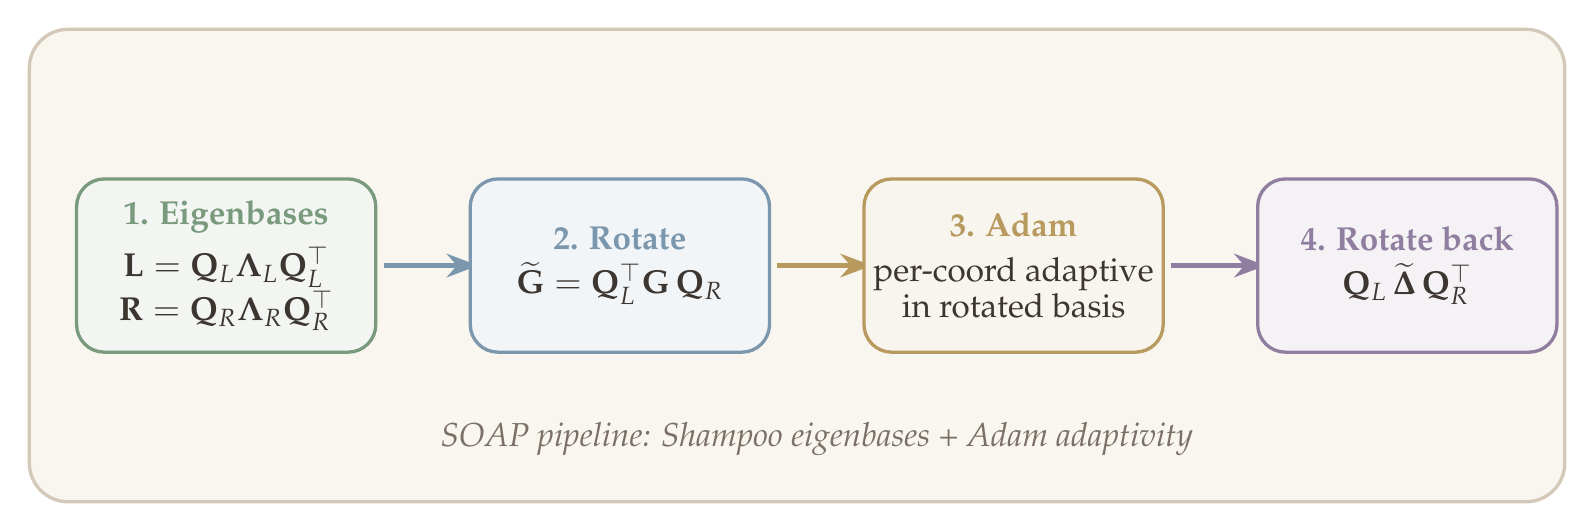
\begin{tikzpicture}[>={Stealth[length=4mm, width=3mm]}, line width=1.5pt]

% Background
\fill[cream, rounded corners=14pt] (-0.5,-1.5) rectangle (19.0,4.5);
\draw[border, line width=1.2pt, rounded corners=14pt] (-0.5,-1.5) rectangle (19.0,4.5);

% Step 1: Eigenbases
\node[draw=sage, line width=1.2pt, fill=sage!10, rounded corners=10pt,
      minimum width=3.8cm, minimum height=2.2cm, align=center, text=dkbrown]
      (step1) at (2.0,1.5) {{\color{sage}\textbf{\large 1. Eigenbases}}\\[4pt]
      {\large $\mathbf{L} = \mathbf{Q}_L \boldsymbol{\Lambda}_L \mathbf{Q}_L^\top$}\\
      {\large $\mathbf{R} = \mathbf{Q}_R \boldsymbol{\Lambda}_R \mathbf{Q}_R^\top$}};

% Arrow 1-2
\draw[stblue, ->, line width=1.5pt] (4.0,1.5) -- (5.2,1.5);

% Step 2: Rotate
\node[draw=stblue, line width=1.2pt, fill=stblue!10, rounded corners=10pt,
      minimum width=3.8cm, minimum height=2.2cm, align=center, text=dkbrown]
      (step2) at (7.0,1.5) {{\color{stblue}\textbf{\large 2. Rotate}}\\[4pt]
      {\large $\widetilde{\mathbf{G}} = \mathbf{Q}_L^\top \mathbf{G}\,\mathbf{Q}_R$}};

% Arrow 2-3
\draw[rwgold, ->, line width=1.5pt] (9.0,1.5) -- (10.2,1.5);

% Step 3: Adam
\node[draw=rwgold, line width=1.2pt, fill=rwgold!10, rounded corners=10pt,
      minimum width=3.8cm, minimum height=2.2cm, align=center, text=dkbrown]
      (step3) at (12.0,1.5) {{\color{rwgold}\textbf{\large 3. Adam}}\\[4pt]
      {\large per-coord adaptive}\\
      {\large in rotated basis}};

% Arrow 3-4
\draw[lavender, ->, line width=1.5pt] (14.0,1.5) -- (15.2,1.5);

% Step 4: Rotate back
\node[draw=lavender, line width=1.2pt, fill=lavender!10, rounded corners=10pt,
      minimum width=3.8cm, minimum height=2.2cm, align=center, text=dkbrown]
      (step4) at (17.0,1.5) {{\color{lavender}\textbf{\large 4. Rotate back}}\\[4pt]
      {\large $\mathbf{Q}_L\,\widetilde{\boldsymbol{\Delta}}\,\mathbf{Q}_R^\top$}};

% Bottom annotation
\node[text=wmgray, font=\large\itshape] at (9.5,-0.7) {SOAP pipeline: Shampoo eigenbases + Adam adaptivity};

\end{tikzpicture}
\end{document}
